\documentclass[nobib]{tufte-handout}
% \documentclass[fleqn,reqno,12pt]{article}

%========================================
% Packages
%========================================

\usepackage[nographicx, nohyperref, nosubcaption, nogb4e]{mfpackages}
\usepackage{mfenvironments}
\usepackage{mfcommands}
% for info boxes
\usepackage{newfloat, caption}
\DeclareCaptionType{InfoBox}


%========================================
% Bibliography
%========================================

\bibliography{references.bib}

%========================================
% General Layout Tweaks
%========================================

% \usepackage[margin=2cm]{geometry}

% Itemize
\renewcommand{\labelitemi}{\large{$\mathbf{\cdot}$}}    % itemize symbols
\renewcommand{\labelitemii}{\large{$\mathbf{\cdot}$}}
\renewcommand{\labelitemiii}{\large{$\mathbf{\cdot}$}}
\renewcommand{\labelitemiv}{\large{$\mathbf{\cdot}$}}
% Description
\renewcommand{\descriptionlabel}[1]{\hspace\labelsep\textsc{#1}}

% Figure Captions
\usepackage{caption} % use corresponding myfiguresize!
\setlength{\captionmargin}{20pt}
\renewcommand{\captionfont}{\small}
\setlength{\belowcaptionskip}{7pt} % standard is 0pt

%========================================
% Define colors and comment functions
%========================================

\usepackage{xcolor}
\definecolor{firebrick}{RGB}{178,34,34}
\definecolor{DarkGreen}{RGB}{34,178,34} 
\definecolor{DarkOrange}{RGB}{255,100,50}
\renewcommand{\mf}[1]{\textcolor{firebrick}{[mf: #1]}}  
\newcommand{\tr}[1]{\textcolor{DarkOrange}{[tr: #1]}}  
%========================================
% Configuring the R code presentation
%========================================

\usepackage{courier}
\usepackage{listings}
\usepackage{color}
% the following defines the layout for the R code
\lstset{ %
  language=R,                     % the language of the code
  basicstyle=\footnotesize\ttfamily, % size and type of the fonts that are used for the code
  numbers=left,                   % where to put the line-numbers
  numberstyle=\tiny\color{gray},  % the style that is used for the line-numbers
  stepnumber=1,                   % the step between two line-numbers. If it's 1, each line
                                  % will be numbered
  numbersep=5pt,                  % how far the line-numbers are from the code
  backgroundcolor=\color{white},  % choose the background color. You must add \usepackage{color}
  showspaces=false,               % show spaces adding particular underscores
  showstringspaces=false,         % underline spaces within strings
  showtabs=false,                 % show tabs within strings adding particular underscores
  frame=single,                   % adds a frame around the code
  rulecolor=\color{black},        % if not set, the frame-color may be changed on line-breaks within not-black text (e.g. commens (green here))
  tabsize=2,                      % sets default tabsize to 2 spaces
  captionpos=b,                   % sets the caption-position to bottom
  breaklines=true,                % sets automatic line breaking
  breakatwhitespace=false,        % sets if automatic breaks should only happen at whitespace
  title=\lstname,                 % show the filename of files included with \lstinputlisting;
                                  % also try caption instead of title
  keywordstyle=\color{blue},      % keyword style
  commentstyle=\color{DarkGreen}, % comment style
  stringstyle=\color{DarkOrange}, % string literal style
  escapeinside={\%*}{*)},         % if you want to add a comment within your code
  morekeywords={*, ...}            % if you want to add more keywords to the set
}

% this is for showing the R output
\lstnewenvironment{rc}[1][]{\lstset{language=R}}{}

% this is for inline R code
\newcommand{\ri}[1]{\lstinline{#1}}  %% Short for 'R inline'

%========================================
% Article Header 
%========================================


\title{Hands-on non-technical tutorial for Bayesian mixed effects regression}
\author{Michael Franke \& Timo Roettger}
\date{}

%========================================
% Article Body
%========================================

\begin{document}
\maketitle

\begin{abstract}
  \noindent Generalized linear mixed models are very versatile and handy tools for statistical inference. Bayesian approaches to applying these models have recently become increasingly popular. This tutorial provides an accessible, non-technical introduction to the use and feel of Bayesian mixed effects regression models. The focus is on data from a factorial-design experiment. \\
  
  \medskip
  
  \noindent \textbf{This tutorial should take you about 1 hour.}
\end{abstract}

\section{Motivation \& intended audience}

This tutorial provides a very basic introduction to Bayesian regression modeling using R \citep{Manual}. We wrote this tutorial with a particular reader in mind. If you have used R before and if you have a basic understanding of linear regression and now you want to find out what a Bayesian approach has to offer, this tutorial is for you. In comparison to other introductions \citep[e.g.][]{SorensenHohensteinb2016:Bayesian-linear}, this tutorial remains very conceptual. We don’t want to ``sell Bayes'' to you, and we do not want to scare you away with mathematical details. We just want to give you an impression of how a Bayesian regression analysis looks and feels. So no reason to be afraid! But also: no reason to be bored, because we \emph{will} cover all the essential concepts and we \emph{will} explain how to run and interpret the output of a Bayesian regression analysis using the wonderful R package \texttt{brms} written by Paul \citet{buerkner2016brms}.

If you don’t have any experience with regression modeling, you will probably still be able to follow but you might also want to consider doing a crash course. To bring you up to speed, we recommend the excellent two-part tutorial by Bodo \citet{Winter2013:Linear-models-a} on mixed effects regression in a non-Bayesian ---a.k.a.~classical or frequentist--- paradigm. In a sense, this tutorial could be considered part three of Bodo's nice and lofty introduction. We will, for example use the same data set.

What you need right now: Please have R \mf{insert URL}) and RStudio \mf{insert URL}) downloaded and installed on your computer.


\section{Our research question}
\label{sec:data}

Imagine we are experimental researchers. Now, what do we do as experimental researchers? We often have a research question about how aspects of nature relate to each other and we want to answer this question. For example, we might want to know whether voice pitch differs across female and male speakers, and whether it differs across social contexts (say: informal and polite contexts). --- To answer our questions, we come up with a nifty experimental design, we lure a group of people into the lab, we ask them to say different words in different social contexts, we record their voices, and extraxt some numbers from these recordings, for example, the pitch values of their voices. We then want to find out whether our data provide evidence for any assumed relationships. So far so good.

In this tutorial, we are looking at data just like this \citep[following[]{Winter2013:Linear-models-a} \citep[taken from][]{WinterGrawunder2012:The-Phonetic-Pr}. You can download the data here: \dots \mf{how to get the data}.  
In order to load the data into R, copy the file \texttt{FILENAME} \dots \mf{describe set up} and type this into an R console (perhaps using RStudio \mf{insert URL})\footnote{If you are familiar with the previous tutorials by \citet{Winter2013:Linear-models-a}, be took the freedom to tidy the data a little bit: we have already removed one line with missing data and we have changed the way the variable
\texttt{scenario} is represented, so that it is treated (correctly) later on in the regression analysis without much further ado.\tr{maybe don't tell them about this? Not relevant for following the tutorial}}

\medskip

\begin{lstlisting}[language=R]
  # load the data into variable 'politedata'
  politedata = read.csv(file = 'MyData.csv')     
\end{lstlisting}

\vspace*{-0.5cm}

\noindent Type \ri{head(politedata)} and you should see the first six lines:

\medskip


\begin{rc}
> head(politedata)
  subject gender scenario attitude  freq
1      F1      F       S1      pol 213.3
2      F1      F       S1      inf 204.5
3      F1      F       S2      pol 285.1
4      F1      F       S2      inf 259.7
5      F1      F       S3      pol 203.9
6      F1      F       S3      inf 286.9
\end{rc}

\medskip

\noindent Looking at the data, we have different subjects. Because voice pitch is highly dependent on gender, we stored whether our subjects are F(emale) or M(ale). Subjects produced words in different scenarios (e.g., words/sentences to pronounce) \tr{maybe we want to rename this column to sentence right away? one less leap to make from data set to concept}. In the experiment, we manipulated whether the scenario took place in a polite or in an informal context. This is indicated by the variable \texttt{attitude}. Crucially, each row contains a measurement of pitch in Hz which is our dependent variable. 

Often, we are interested in comparing a dependent variable (here pitch) across different conditions or groups, i.e. independent variables. Before our data collection, we might have formulated concrete predictions about the relationship between the dependent variable and independent variables. For example, we might have formulated the following three hypotheses:

\begin{enumerate}[{H}1:]
\item Female speakers have a lower average pitch in polite than in informal contexts.
\item Male speakers have a lower average pitch in polite than in informal contexts.
\item Male speakers have a lower average pitch in informal than female speakers have in polite contexts.
\end{enumerate}

\noindent Maybe you are interested in other pairwise relationships, maybe you are interested in main effects of gender or attitude regardless of the other groupings. For exposition purposes, let's just go with these arbitrarily chosen hypotheses.

To get a first idea of possible relationships in our data, let's plot them. Figure~\ref{fig:BasicPlotData_data} displays the mean pitch values for each scenario (semitransparent points) across gender and attitude; The solid points indicate the mean pitch values across gender and attitude. Looking at the plot, we can see that pitch values from female speakers are generally higher than values from male speakers (points in left column are higher than in the right column). We also see that pitch values in the informal condition are slightly higher than those in the polite condition (blue points are slightly higher than orange points). 

Intuitively, these patterns might strike us as pretty obvious, but there is also quite a lot of variability between scenarios. For example, some values from the informal condition for female speakers (blue points in left column), are lower than their corresponding polite counterparts.  
What we want is a precise estimates of potential differences between groups alongside a measure of certainty around these estimates. 

\tr{agree with getting rid of simple plotting explanations, so delete code chunk?}. 

\medskip

\begin{lstlisting}[language=R]
# load a package for data wrangling and plotting
library(tidyverse)
# load a package to obtain function 'std.error' for standard errors
library(plotrix)
# plot means for each group
politedata %>% 
  group_by(gender, attitude) %>% 
  summarize(mean_frequency = mean(freq),
            standard_error = std.error(freq)) %>% 
  ggplot((aes(x = gender, 
              y = mean_frequency, 
              fill = attitude))) + 
  geom_bar(stat = "identity", position = "dodge") +
  geom_errorbar(aes(ymin = mean_frequency - standard_error,
                    ymax = mean_frequency + standard_error), 
                    position = "dodge")
\end{lstlisting}


\begin{figure}[t]
  \centering
    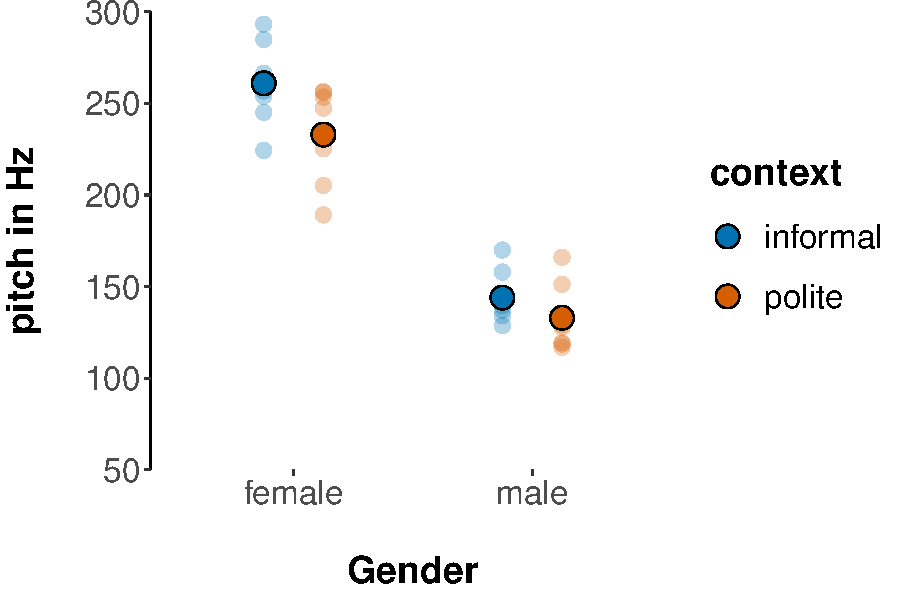
\includegraphics[width = \textwidth]{pics/basic_data_plot.pdf}
    \caption{Basic plot of the data.}
     \label{fig:BasicPlotData_data}
\end{figure}

Another way of looking at the data in connection with our research hypotheses is in Figure~\ref{fig:BasicPlotData_table}. Each cell represent one unique combination of the gender and the attitude factor. Our hypotheses can be related to the comparison between some of these cells. H1 makes a statement about the comparison between quadrant 1 and 2 (the attitude effect for female speakers); H2 makes a statement about quadrant 3 and 4 (the attitude effect for male speakers); and H3 makes a statement about quadrant 2 and 3 (the difference between informal male speakers and polite female speakers).

\begin{figure}[h]
  \centering
    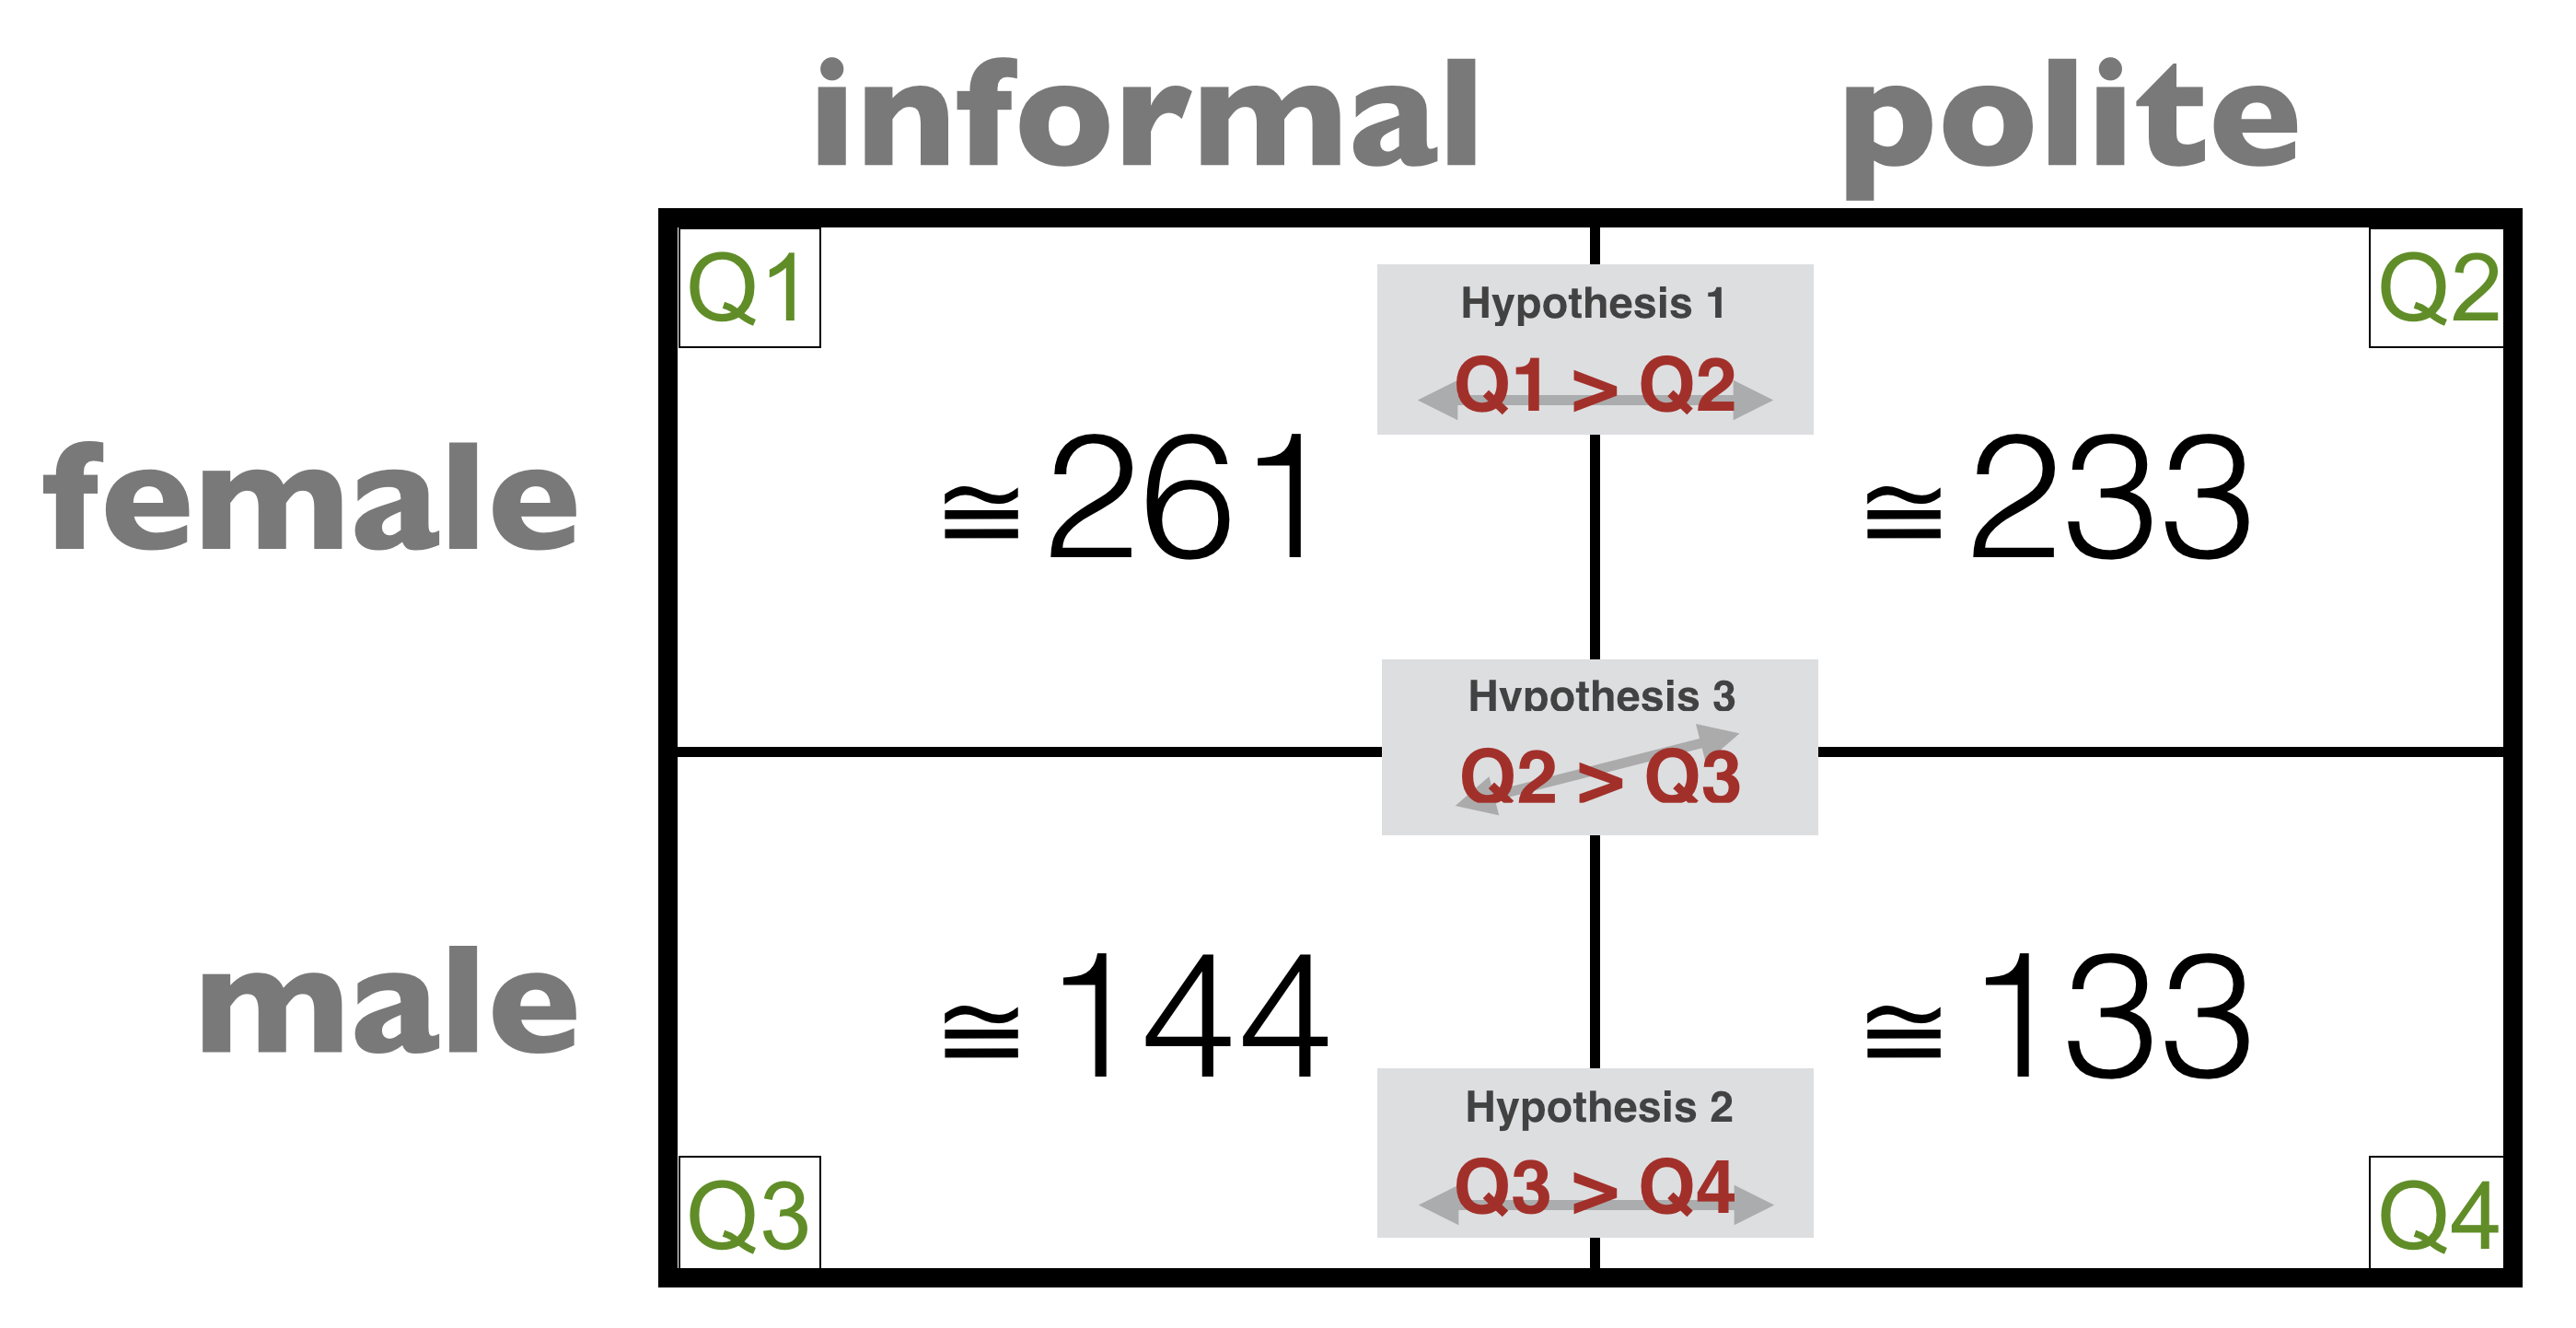
\includegraphics[width = \textwidth]{pics/table_mean_hypotheses.png}
    \caption{Means of each design cell \& research hypotheses.}
    \label{fig:BasicPlotData_table}
\end{figure}

\mf{Next steps: give the table of means; say how above comparisons translate into a comparison of cells in that table}

Within the bayesian framework, we can estimate the values for each cell and, in turn, the differences between cells directly. Our aim is to get some values about voice pitch for males and females and polite and informal contexts. 

We can express the relationship between pitch on the one hand and gender and attitude on the other as a regression formula like this one here: pitch ~ gender * attitude.

Translated into the syntax of brms we end up with following function:

\medskip

\begin{lstlisting}[language=R]
  # formulate regression model in brms
  xmdl = brm(freq ~ gender * attitude, data = politedata)
\end{lstlisting}

\vspace*{-0.5cm}

\noindent 

The syntax of this function should look very familiar to anyone who has worked with (generalized) linear models in R. Now one important difference between traditional frequentist' inferences and a Bayesian framework is that we can take specific prior beliefs about the relationships between dependent and independent variables into account. 

Priors are subjective pieces of information about your data that you have before analyzing the data. These priors might constrain values that your data can have. For example, mathematically, pitch values  cannot be lower than 0. Practically, human pitch values are within a certain range that is limited by bio mechanical constraints on our laryngeal system. In adults, values beyond, let's say 1000 Hz are very unlikely even when they use falsetto.
Priors can also express our subjective beliefs about a relationship. For example, knowing what we know about gender differences in pitch, we might be already very certain that female speakers have higher pitch values than male speakers.

But wait a minute. Subjective beliefs? This is science. We are supposed to be objective, right? You are right. Although, they are cases in which we might want to specify very concrete priors about our data, practically we will restrict ourselves here to what we call weakly informative priors. Weakly informative priors are priors that constrain possible values of a variable (e.g. possible pitch values). These priors are also called regularizing priors, as they help the statistical model to converge on reasonable estimates. But these priors are also agnostic about possible relationships between variables. 



\tr{Below is stuff to mention when we transition to hierarchical models}. 

These mean values, however, are a very poor and abstract representation of all the pitch values that we have recorded. Different speakers have very different voice pitch ranges. Likewise, speakers are not machines. There is a substantial variability in how a single speaker pronounces an utterance. So we expect some variability here. Likewise,
different scenarios might elicit very different pitch values due idiosyncratic aspects of the scenario that are not captured by our independent variables. 

In our study, we took multiple measures per speaker. That is, each subject gave multiple polite responses and multiple informal responses. 
Individual responses from one subject are thus dependent. Also, we took multiple measures per scenario, as each scenario was produced by all speakers. This introduces, again, dependencies between data points. These dependencies need to be taken into account when we try to estimate differences between groups.


\newpage

\begin{InfoBox}[t]
\centering
\colorbox{mygray}{\centering
  \begin{minipage}{1.0\textwidth}

    \emph{Bayesian inference: priors, likelihoods and posteriors}
    \medskip

    Jones is a rational scientist. She has recently inherited her grandma's lucky coin. Grandma
    used this coin many times during Jones' childhood to determine whether Jones was allowed a
    sweet or not. Jones suspects that grandma's coin might be a trick coin, but she is not
    sure. She is determined to find out. How? Well, naturally, by rationally updating her
    \emph{prior beliefs} about the coin's bias to obtain a new \emph{posterior belief} based on
    empirical observation (outcomes of coin flips). Central to this updating is Jones'
    \emph{likelihood function}, which encodes how likely each relevant coin bias may have
    generated the observed data. --- Sounds fancifully abstract? It's actially fairly intuitive.
    Consider this example.
    
    \paragraph{Prior beliefs.} Jones initially believes that the coin is either biased towards
    heads or biased towards tails, and that both of these possibilities are equally likely. She
    also believes that, if biased towards heads, the coin is three times more likely to come up
    heads; and that, if biased towards tails, the coin is three times more likely to come up
    tails. Numerically, Jones' \emph{prior beliefs} can be written as, where $\theta \in [0;1]$
    is the coin's bias: $P(\theta = \nicefrac{1}{3}) = \nicefrac{1}{2}$, and $P(\theta =
    \nicefrac{2}{3}) = \nicefrac{1}{2}$.

    \paragraph{Likelihood.} The bias $\theta$ is, by definition, the probability of the coin
    landing heads on the next trial. Let's assume that Jones tosses the coin only once (hm,
    maybe not so rational a scientist after all? or just too busy?). Let $D$ be the set of
    potential outcomes of this experiment, namely $D = \set{\text{heads}, \text{tails}}$. The
    \emph{likelihood function} determines the likelihood of observing each datum $d \in D$ for
    each $\theta$, which in our case is just rather trivial: $P(D = \text{heads} \mid \theta) =
    \theta$ and $P(D = \text{tails} \mid \theta) = 1 - \theta$.

    \paragraph{Posterior beliefs.} Jones observes that the coin landed heads. What should she
    believe now. By \emph{Bayes rule} her posterior beliefs are defined like so:
    \begin{align*}
      P(\theta \mid D = \text{heads}) = \frac{P(\theta) P(D = \text{heads} \mid \theta)}{\sum_{\theta'}P(\theta') P(D = \text{heads} \mid \theta')}
    \end{align*}
    Jones' posterior belief that the coin is twice as likely to land heads is therefore:
    \begin{align*}
      P(\theta = \nicefrac{2}{3} \mid D = \text{heads}) & = \frac{P(\theta = \nicefrac{2}{3}) \ P(D = \text{heads} \mid \theta = \nicefrac{2}{3})}{P(\theta = \nicefrac{2}{3}) \ P(D = \text{heads} \mid \theta = \nicefrac{2}{3}) + P(\theta = \nicefrac{1}{3}) \ P(D = \text{heads} \mid \theta = \nicefrac{1}{3})} \\
            & = \frac{\nicefrac{1}{2} \ \nicefrac{2}{3}}{\nicefrac{1}{2} \ \nicefrac{2}{3} + \nicefrac{1}{2} \ \nicefrac{1}{3}} = \nicefrac{1}{2}
    \end{align*}
    After making her observation, rational Jones believes that the bias towards heads is twice
    more likely than the bias towards tails.
    
    \tr{I think this will make everyone run away from this tutorial. Can we keep it on a pure conceptual level and avoid any formulas?}. 

  \end{minipage} \par
  } \par
  \begin{center}
    Info Box 1: Priors, likelihood and posteriors in Bayesian inference.
  \end{center}
  % \caption{\label{InfoBox:asymptotic_CIs} Here is my caption}  
\end{InfoBox}






\printbibliography[heading=bibintoc]

\end{document}
